\documentclass[twoside]{book}

% Packages required by doxygen
\usepackage{fixltx2e}
\usepackage{calc}
\usepackage{doxygen}
\usepackage[export]{adjustbox} % also loads graphicx
\usepackage{graphicx}
\usepackage[utf8]{inputenc}
\usepackage{makeidx}
\usepackage{multicol}
\usepackage{multirow}
\PassOptionsToPackage{warn}{textcomp}
\usepackage{textcomp}
\usepackage[nointegrals]{wasysym}
\usepackage[table]{xcolor}

% Font selection
\usepackage[T1]{fontenc}
\usepackage[scaled=.90]{helvet}
\usepackage{courier}
\usepackage{amssymb}
\usepackage{sectsty}
\renewcommand{\familydefault}{\sfdefault}
\allsectionsfont{%
  \fontseries{bc}\selectfont%
  \color{darkgray}%
}
\renewcommand{\DoxyLabelFont}{%
  \fontseries{bc}\selectfont%
  \color{darkgray}%
}
\newcommand{\+}{\discretionary{\mbox{\scriptsize$\hookleftarrow$}}{}{}}

% Page & text layout
\usepackage{geometry}
\geometry{%
  a4paper,%
  top=2.5cm,%
  bottom=2.5cm,%
  left=2.5cm,%
  right=2.5cm%
}
\tolerance=750
\hfuzz=15pt
\hbadness=750
\setlength{\emergencystretch}{15pt}
\setlength{\parindent}{0cm}
\setlength{\parskip}{3ex plus 2ex minus 2ex}
\makeatletter
\renewcommand{\paragraph}{%
  \@startsection{paragraph}{4}{0ex}{-1.0ex}{1.0ex}{%
    \normalfont\normalsize\bfseries\SS@parafont%
  }%
}
\renewcommand{\subparagraph}{%
  \@startsection{subparagraph}{5}{0ex}{-1.0ex}{1.0ex}{%
    \normalfont\normalsize\bfseries\SS@subparafont%
  }%
}
\makeatother

% Headers & footers
\usepackage{fancyhdr}
\pagestyle{fancyplain}
\fancyhead[LE]{\fancyplain{}{\bfseries\thepage}}
\fancyhead[CE]{\fancyplain{}{}}
\fancyhead[RE]{\fancyplain{}{\bfseries\leftmark}}
\fancyhead[LO]{\fancyplain{}{\bfseries\rightmark}}
\fancyhead[CO]{\fancyplain{}{}}
\fancyhead[RO]{\fancyplain{}{\bfseries\thepage}}
\fancyfoot[LE]{\fancyplain{}{}}
\fancyfoot[CE]{\fancyplain{}{}}
\fancyfoot[RE]{\fancyplain{}{\bfseries\scriptsize Generated by Doxygen }}
\fancyfoot[LO]{\fancyplain{}{\bfseries\scriptsize Generated by Doxygen }}
\fancyfoot[CO]{\fancyplain{}{}}
\fancyfoot[RO]{\fancyplain{}{}}
\renewcommand{\footrulewidth}{0.4pt}
\renewcommand{\chaptermark}[1]{%
  \markboth{#1}{}%
}
\renewcommand{\sectionmark}[1]{%
  \markright{\thesection\ #1}%
}

% Indices & bibliography
\usepackage{natbib}
\usepackage[titles]{tocloft}
\setcounter{tocdepth}{3}
\setcounter{secnumdepth}{5}
\makeindex

% Hyperlinks (required, but should be loaded last)
\usepackage{ifpdf}
\ifpdf
  \usepackage[pdftex,pagebackref=true]{hyperref}
\else
  \usepackage[ps2pdf,pagebackref=true]{hyperref}
\fi
\hypersetup{%
  colorlinks=true,%
  linkcolor=blue,%
  citecolor=blue,%
  unicode%
}

% Custom commands
\newcommand{\clearemptydoublepage}{%
  \newpage{\pagestyle{empty}\cleardoublepage}%
}

\usepackage{caption}
\captionsetup{labelsep=space,justification=centering,font={bf},singlelinecheck=off,skip=4pt,position=top}

%===== C O N T E N T S =====

\begin{document}

% Titlepage & ToC
\hypersetup{pageanchor=false,
             bookmarksnumbered=true,
             pdfencoding=unicode
            }
\pagenumbering{alph}
\begin{titlepage}
\vspace*{7cm}
\begin{center}%
{\Large My Project }\\
\vspace*{1cm}
{\large Generated by Doxygen 1.8.13}\\
\end{center}
\end{titlepage}
\clearemptydoublepage
\pagenumbering{roman}
\tableofcontents
\clearemptydoublepage
\pagenumbering{arabic}
\hypersetup{pageanchor=true}

%--- Begin generated contents ---
\chapter{Class Index}
\section{Class List}
Here are the classes, structs, unions and interfaces with brief descriptions\+:\begin{DoxyCompactList}
\item\contentsline{section}{\hyperlink{structEnigme}{Enigme} }{\pageref{structEnigme}}{}
\end{DoxyCompactList}

\chapter{File Index}
\section{File List}
Here is a list of all documented files with brief descriptions\+:\begin{DoxyCompactList}
\item\contentsline{section}{{\bfseries enigme.\+h} }{\pageref{enigme_8h}}{}
\item\contentsline{section}{\hyperlink{main_8c}{main.\+c} \\*Testing Program }{\pageref{main_8c}}{}
\end{DoxyCompactList}

\chapter{Class Documentation}
\hypertarget{structEnigme}{}\section{Enigme Struct Reference}
\label{structEnigme}\index{Enigme@{Enigme}}
\subsection*{Public Attributes}
\begin{DoxyCompactItemize}
\item 
\mbox{\Hypertarget{structEnigme_a4cd8d8e0cb1572ed1f34f17b7c9d5936}\label{structEnigme_a4cd8d8e0cb1572ed1f34f17b7c9d5936}} 
S\+D\+L\+\_\+\+Surface $\ast$ {\bfseries background} \mbox{[}2\mbox{]}
\item 
\mbox{\Hypertarget{structEnigme_a9461c400dca33109161b4e274665623f}\label{structEnigme_a9461c400dca33109161b4e274665623f}} 
S\+D\+L\+\_\+\+Surface $\ast$ {\bfseries boutons} \mbox{[}5\mbox{]}
\item 
\mbox{\Hypertarget{structEnigme_ac9591e5cf1c5ed6bd3aafde9dcac1abe}\label{structEnigme_ac9591e5cf1c5ed6bd3aafde9dcac1abe}} 
S\+D\+L\+\_\+\+Surface $\ast$ {\bfseries reponses} \mbox{[}5\mbox{]}
\item 
\mbox{\Hypertarget{structEnigme_ade179239287a8895af3b03645401f42d}\label{structEnigme_ade179239287a8895af3b03645401f42d}} 
S\+D\+L\+\_\+\+Surface $\ast$ {\bfseries question}
\item 
\mbox{\Hypertarget{structEnigme_a59e8d5c6333aaed6c6b7f611283897f7}\label{structEnigme_a59e8d5c6333aaed6c6b7f611283897f7}} 
S\+D\+L\+\_\+\+Surface $\ast$ {\bfseries win}
\item 
\mbox{\Hypertarget{structEnigme_ab26b2e7b5c20c0941127162ae81222d7}\label{structEnigme_ab26b2e7b5c20c0941127162ae81222d7}} 
S\+D\+L\+\_\+\+Surface $\ast$ {\bfseries lost}
\item 
\mbox{\Hypertarget{structEnigme_a919ddc72bc942752bb0ed286d562781b}\label{structEnigme_a919ddc72bc942752bb0ed286d562781b}} 
S\+D\+L\+\_\+\+Rect {\bfseries pos\+Repones} \mbox{[}5\mbox{]}
\item 
\mbox{\Hypertarget{structEnigme_aa2e04f02c23d489994e4834313a90ec8}\label{structEnigme_aa2e04f02c23d489994e4834313a90ec8}} 
S\+D\+L\+\_\+\+Rect {\bfseries pos\+Question}
\item 
\mbox{\Hypertarget{structEnigme_a173ec8a7cd7b2afdecabae655a3d62f2}\label{structEnigme_a173ec8a7cd7b2afdecabae655a3d62f2}} 
int {\bfseries choix\+\_\+question}
\item 
\mbox{\Hypertarget{structEnigme_a9e63249d7a05e0e4c6c3d6446afeef05}\label{structEnigme_a9e63249d7a05e0e4c6c3d6446afeef05}} 
int {\bfseries image\+\_\+courrante}
\item 
\mbox{\Hypertarget{structEnigme_a35df3bcc2d86e77715bbaae99ac58217}\label{structEnigme_a35df3bcc2d86e77715bbaae99ac58217}} 
int {\bfseries position\+Vrai\+Reponse}
\end{DoxyCompactItemize}


The documentation for this struct was generated from the following file\+:\begin{DoxyCompactItemize}
\item 
enigme.\+h\end{DoxyCompactItemize}

\chapter{File Documentation}
\hypertarget{main_8c}{}\section{main.\+c File Reference}
\label{main_8c}\index{main.\+c@{main.\+c}}


Testing Program.  


{\ttfamily \#include $<$stdio.\+h$>$}\newline
{\ttfamily \#include $<$stdlib.\+h$>$}\newline
{\ttfamily \#include \char`\"{}enigme.\+h\char`\"{}}\newline
Include dependency graph for main.\+c\+:
\nopagebreak
\begin{figure}[H]
\begin{center}
\leavevmode
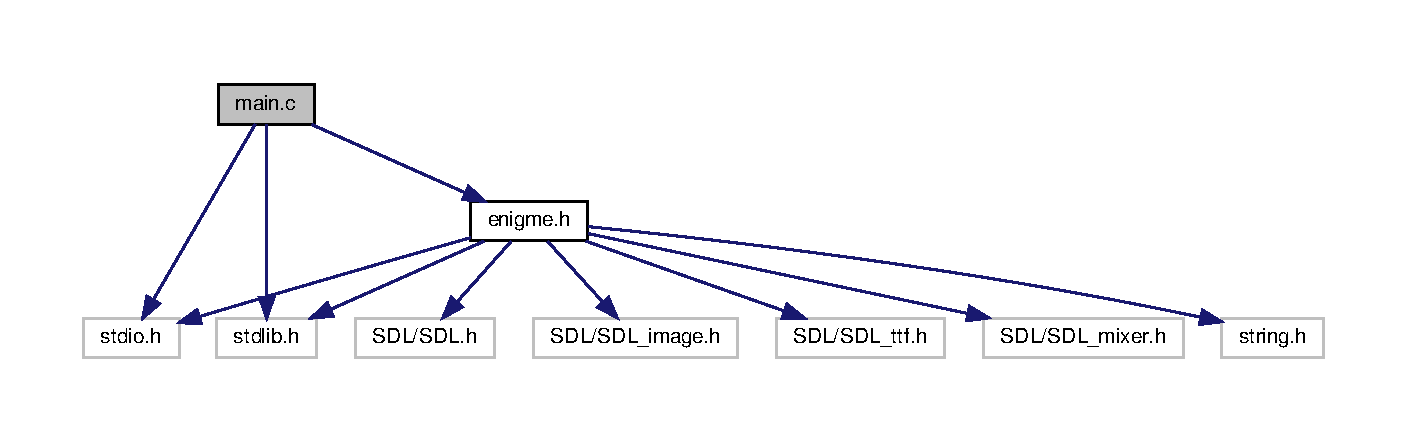
\includegraphics[width=350pt]{main_8c__incl}
\end{center}
\end{figure}
\subsection*{Functions}
\begin{DoxyCompactItemize}
\item 
\mbox{\Hypertarget{main_8c_ae66f6b31b5ad750f1fe042a706a4e3d4}\label{main_8c_ae66f6b31b5ad750f1fe042a706a4e3d4}} 
int {\bfseries main} ()
\end{DoxyCompactItemize}


\subsection{Detailed Description}
Testing Program. 

\begin{DoxyAuthor}{Author}
C Team 
\end{DoxyAuthor}
\begin{DoxyVersion}{Version}
0.\+1 
\end{DoxyVersion}
\begin{DoxyDate}{Date}
Apr 01, 2015
\end{DoxyDate}
Testing program for background scrollilng 
%--- End generated contents ---

% Index
\backmatter
\newpage
\phantomsection
\clearemptydoublepage
\addcontentsline{toc}{chapter}{Index}
\printindex

\end{document}
